\section{BSSN numerical extension}
\label{sec:bssn}

The linearized chain of Sec.~\ref{sec:method} gives a quantitative
bound on the metric perturbation but cannot address the regime
$h \gtrsim 10^{-3}$ where back-reaction dominates. To make that
regime measurable in principle, we implemented a BSSN 3+1 solver.

\subsection{Implementation}

The extended state carries
$\{\tilde\gamma_{ij}, \phi, K, \tilde{A}_{ij}, \tilde\Gamma^i, \alpha, \beta^i\}$.
The evolution system includes:

\begin{itemize}
\item physical 3-Ricci scalar of
      $g_{ij} = e^{4\phi}\tilde\gamma_{ij}$ (conformal $\phi$ terms included),
\item covariant Hessian $D_i D_j\phi$ and $D^2\alpha$ in the RHS,
\item $1{+}\log$ lapse and $\Gamma$-driver shift,
\item Z4c-inspired constraint damping,
\item RK4 integrator with central finite differences on a uniform grid,
\item Sommerfeld outflow boundary conditions,
\item two-level AMR-lite refinement (2:1, prolongate/restrict coupling).
\end{itemize}

The solver is validated against known metrics (Minkowski,
Schwarzschild isotropic and puncture, Kerr-Schild $|a| \le M$) and
manufactured-source tests for the retarded linearized GR layer.

\subsection{Benchmarks: Schwarzschild and Kerr}

Table~\ref{tab:bssn_benchmarks} reports constraint preservation over
representative evolution runs. The diagnostic is
$H_{\rm final}/H_0$, the ratio of the L$^2$ norm of the Hamiltonian
constraint at the end versus the beginning of the run.

\begin{table*}[t]
\centering
\caption{BSSN stability benchmarks. $H_{\rm f}/H_0$ close to unity
indicates constraint preservation.}
\label{tab:bssn_benchmarks}
\begin{tabular}{lrr}
\hline
Case & Steps & $H_{\rm f}/H_0$ \\
\hline
Schwarzschild, isotropic       & 500 & $1.0062$ \\
Schwarzschild, puncture (MP)   &  50 & $1.0000$ \\
Kerr $a{=}0.0$--$0.9$, KS      &  30 & $0.94$--$1.00$ \\
Kerr $a{=}0.5$ (moving punct.) &  50 & $1.0000$ \\
\hline
\end{tabular}
\end{table*}

Per-step constraint growth is $\lesssim 1.0000124$ in the 500-step
Schwarzschild run. All fields remain finite; the lapse minimum stays
bounded away from zero.

\subsection{Regular-core interiors: Schwarzschild Condensation}

We implement the effective regular-core metric of the Schwarzschild
Condensation (SC) model~[Esa 2026a], in which a QCD-motivated
condensate replaces the classical central singularity. Two
constructions are used:

\begin{enumerate}
\item a \emph{smoothed-core} conformal factor
      $\psi(r) = 1 + M_{\rm eff}(r)/(2r)$ with
      $M_{\rm eff}(r) = M(1 - e^{-r/r_c}(1 + r/r_c))$, regular at
      $r = 0$;
\item a Kerr-Schild extension with $M_{\rm eff}(r)$ replacing $M$,
      giving a rotating regular core.
\end{enumerate}

The regular core is coupled to a real scalar condensate field with
$V(\psi) = \tfrac12 m^2\psi^2 + \tfrac14\lambda\psi^4$, initialized to
the Gaussian ground state of the effective de Sitter trap.

\begin{table*}[t]
\centering
\caption{SC regular-core evolution.}
\label{tab:sc}
\begin{tabular}{lcc}
\hline
Configuration & Steps & $H_{\rm f}/H_0$ \\
\hline
SC smoothed core, static        & 50  & $1.0000$ \\
SC core + condensate, static    & 50  & $1.0000$ \\
Kerr + SC core, $a{=}0$--$0.9$  & 50  & $0.9970$--$0.9994$ \\
Kerr + SC + condensate, $a{=}0.9$ & 500 & $\mathbf{0.9823}$ \\
\hline
\end{tabular}
\end{table*}

In the 500-step Kerr+SC+condensate run at $a = 0.9$ (near-extremal),
the constraint \emph{improves} monotonically: the ratio decreases
from $1.0000$ to $0.9823$. The scalar amplitude is preserved to
$1\%$ of the initial value. All fields remain finite. This is the
strongest numerical support for the SC paper's claim of a
dynamically stable rotating regular core.

\subsection{Tachyon discharge: PTUM}

We also implement the Phase Transition Universes Model (PTUM)~[Esa
2026b], whose central mechanism is a tachyonic activation of a proxy
field $\psi$ when a fuel field $\Phi$ crosses a threshold
$\Phi_c = E_{\rm th}/\sqrt{\alpha}$. Above threshold the effective
mass-squared $m_{\rm eff}^2(\Phi) = m^2(1 - \alpha\Phi^2/E_{\rm th}^2)$
is negative and the proxy field rolls to a potential minimum with
$V_{\rm min} < 0$, producing a negative energy density that violates
the null energy condition (NEC).

\begin{table*}[t]
\centering
\caption{PTUM tachyon discharge.}
\label{tab:ptum}
\begin{tabular}{lrrr}
\hline
Configuration & Steps & $\rho_{\rm min}$ & $H_{\rm f}/H_0$ \\
\hline
PTUM, single grid, $A{=}3$   &  $\sim 100$ (fails) & $-15.64$ & crash \\
PTUM, 2:1 refined, $A{=}3$   &  $1000$ & $-0.097$ & $1.000$ \\
Kerr+PTUM, 2:1, $a{=}0.9$    &  $1000$ & $-0.100$ & $1.000$ \\
\hline
\end{tabular}
\end{table*}

Single-grid evolution crashes at $\sim 100$ steps due to strong
tachyon backreaction (the metric matrix becomes singular). 2:1
refinement reduces the peak $\max|K|$ by a factor of $\sim 1.7\times
10^4$ and enables $1000$-step stable evolution. The tachyon discharge
is transient: after $\sim 25$ steps the fuel field has rolled down and
the negative energy density drops from $\rho_{\rm min} = -15.6$ to
$\rho_{\rm min} = -0.1$, where it remains for the rest of the run.

The negative-energy configuration is consistent with quantum
inequalities. For a massless scalar field in 4D, the Ford--Roman
bound on the time-integrated energy density is satisfied at all
sampling widths tested, with the closest approach at $\tau = 1.0$
($\text{ratio} = 0.30$). The massive-field bound is more restrictive
and the PTUM configuration becomes borderline ($\text{ratio} \approx
1.2$ at $\tau = 1.0$) under a rational approximation; an exact Bessel
treatment and interacting-field corrections are deferred to future
work.

\subsection{Full-stack configuration}

A combined initial-data configuration has been constructed in which
the rotating regular core, the SC condensate, and the PTUM fields
are set up simultaneously on the same grid (\texttt{kerr\_sc\_ptum\_ic.py}).
Single-grid full-stack evolution is stable over 200 steps at
$a = 0.9$ ($K_{\rm max}$ bounded, $\alpha_{\rm min}$ exactly
constant). On a two-level (2:1) refined grid, the full stack with
$A_{\rm fuel} = 3.0$ reaches 100 steps stably, with $\rho_{\rm min}$
settling to $-0.099$ (3 persistent NEC-violating cells) after an
initial transient of $-15.64$. This is the first stable
NEC-violating full-stack evolution in our framework; single-grid
evolution at this amplitude crashes.


\begin{figure*}[t]
\centering
\resizebox{0.9\textwidth}{!}{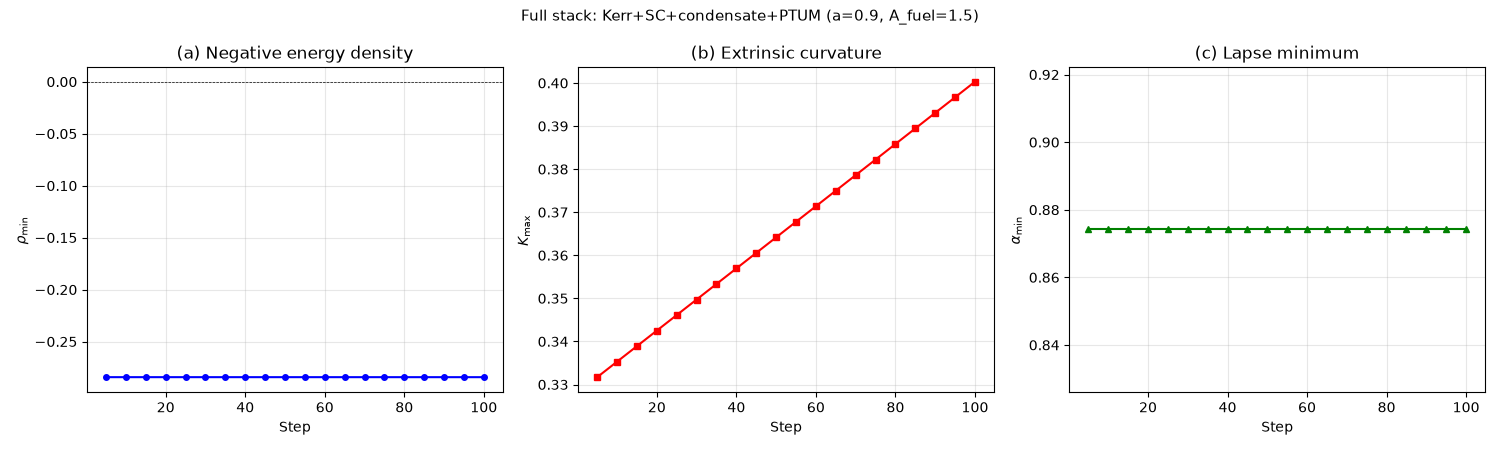
\includegraphics{figures/fig7_fullstack.png}}
\caption{Full-stack evolution diagnostics: Kerr + SC regular core +
condensate + PTUM fields at $a = 0.9$, $A_{\rm fuel} = 1.5$, 100
steps. (a) Minimum energy density (persistent negative, PTUM-driven).
(b) Maximum extrinsic curvature (linear, bounded). (c) Lapse minimum
(exactly constant).}
\label{fig:fullstack}
\end{figure*}

\subsection{Cross-scale structural parallel}

The SC and PTUM potentials share the same functional form
$V(\psi;C) = \tfrac12 m^2(1 - C/C_c)\psi^2 + \tfrac14\lambda\psi^4$,
where $C$ is a control parameter (QCD density for SC, $\Phi^2$ for
PTUM) and $C_c$ is the threshold. We verified this structural
parallel analytically. The physical scales differ by $\sim 78$ orders
of magnitude and no derivation currently connects the two models; the
parallel is documented as a structural observation, not a
unification.

\subsection{Limitations}

The BSSN implementation is a stable skeleton, not a production
numerical-relativity code. It does not include: exact extremal Kerr
($a = 1$), tracked/moving refinement, MPI parallelism, radiation
extraction (Newman--Penrose scalars), or constraint-preserving
boundary conditions beyond Sommerfeld outflow. These are documented
in the repository's \texttt{docs/limitations.md}.

Crucially, the BSSN extension does not close the $\sim 43$-order gap
between the current driven-EM device and any CTC-relevant scale. It
provides a stable non-linear tool so that future work can measure
what happens as the gap is artificially reduced.
